%----------------------------------------------------------------------------------------
%	PACKAGES AND THEMES
%----------------------------------------------------------------------------------------
\documentclass[11pt]{beamer}
\usepackage[utf8]{inputenc}
\usepackage[T1]{fontenc}
\usepackage[italian,english]{babel}
\usepackage{graphicx}
\usepackage{tikz}
\usepackage{pifont}
\usepackage{amsmath,amsthm}
\usepackage{amsfonts}
\usepackage{graphicx}
\usepackage{adjustbox}
\usepackage{float,subfloat}
\usepackage{wrapfig}
\usepackage{lipsum}
\usepackage{bbm}
\usepackage{bm}
\usepackage{empheq}
\usepackage{mathtools}
\usepackage{algorithm,algpseudocode}
\usepackage{booktabs,longtable}
\usepackage{array}
\usetheme{Warsaw}
\usecolortheme{orchid}
%\setbeamerfont{frametitle}{size=\Large}
%\setbeamertemplate{frametitle}

\DeclareMathOperator*{\Optmax}{max}
%----------------------------------------------------------------------------------------
%	TITLE PAGE
%----------------------------------------------------------------------------------------

\title[] % (optional, only for long titles)
{\huge A Stochastic Reachability Approach to Asset Allocation.}
\subtitle{\Large From time-based to event-driven systematic strategies.}
\author[] % (optional, for multiple authors)
{Andrea Schiavon\\
	andrea.schiavon1992@gmail.com}

\date[]{\today} % (optional)

\AtBeginSection[]{
	\begin{frame}
		\vfill
		\centering
		\begin{beamercolorbox}[sep=8pt,center,shadow=true,rounded=true]{title}
			\usebeamerfont{title}\insertsectionhead\par%
		\end{beamercolorbox}
		\vfill
	\end{frame}
}	
\begin{document}


\begin{frame}[plain]
	\begin{figure}[htpb]
		\centering
		
\includegraphics[width=0.4\linewidth]{Images/polimi_name}
	\end{figure}
	\titlepage
\end{frame}


%----------------------------------------------------------------------------------------
%	INTRODUZIONE
%---------------------------------------------------------------------------------------
\begin{frame}{Che cos'è l'Asset Allocation?}
	
    \begin{definition}
			L’\textbf{asset allocation} è il processo con il quale si decide in che modo distribuire le risorse fra diversi i possibili investimenti
    \end{definition}
	\begin{figure}
		\centering
		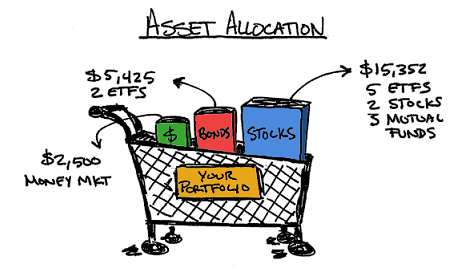
\includegraphics[width=.6\linewidth]{Images/AA}
	\end{figure}
\end{frame}


\begin{frame}{Raggiungibilità Stocastica: un esempio di applicazione}
	\begin{block}{Gestione del Traffico Aereo}
		\begin{figure}
			\centering
			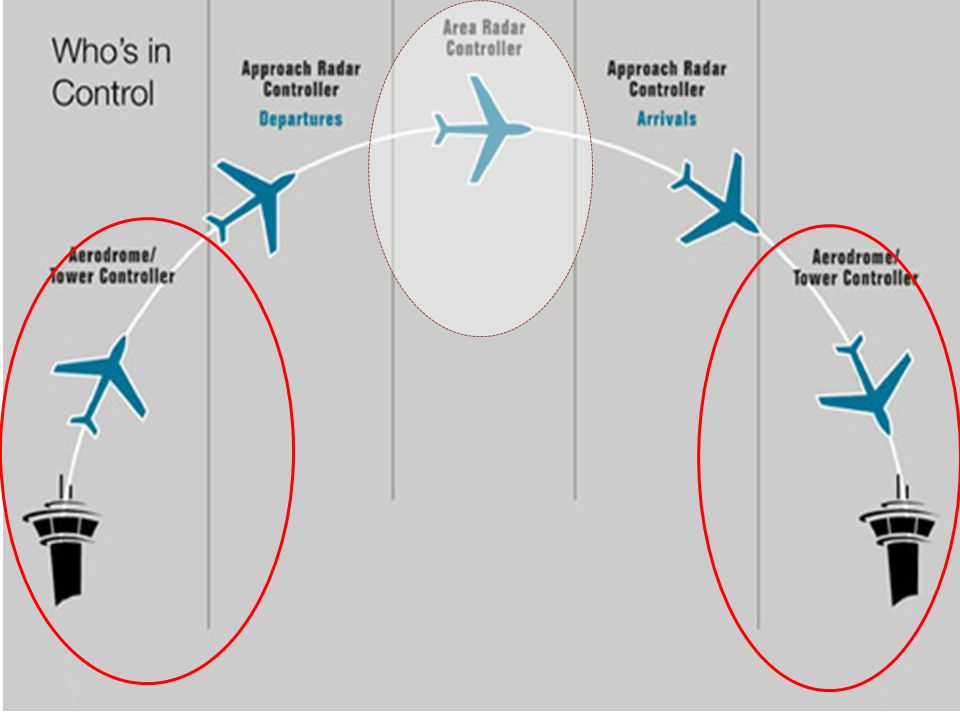
\includegraphics[width=0.7\linewidth]{Images/ATM}
		\end{figure}
	\end{block}
\end{frame}
\begin{frame}{Raggiungibilità Stocastica in Finanza}
	
		\begin{figure}
			\centering
			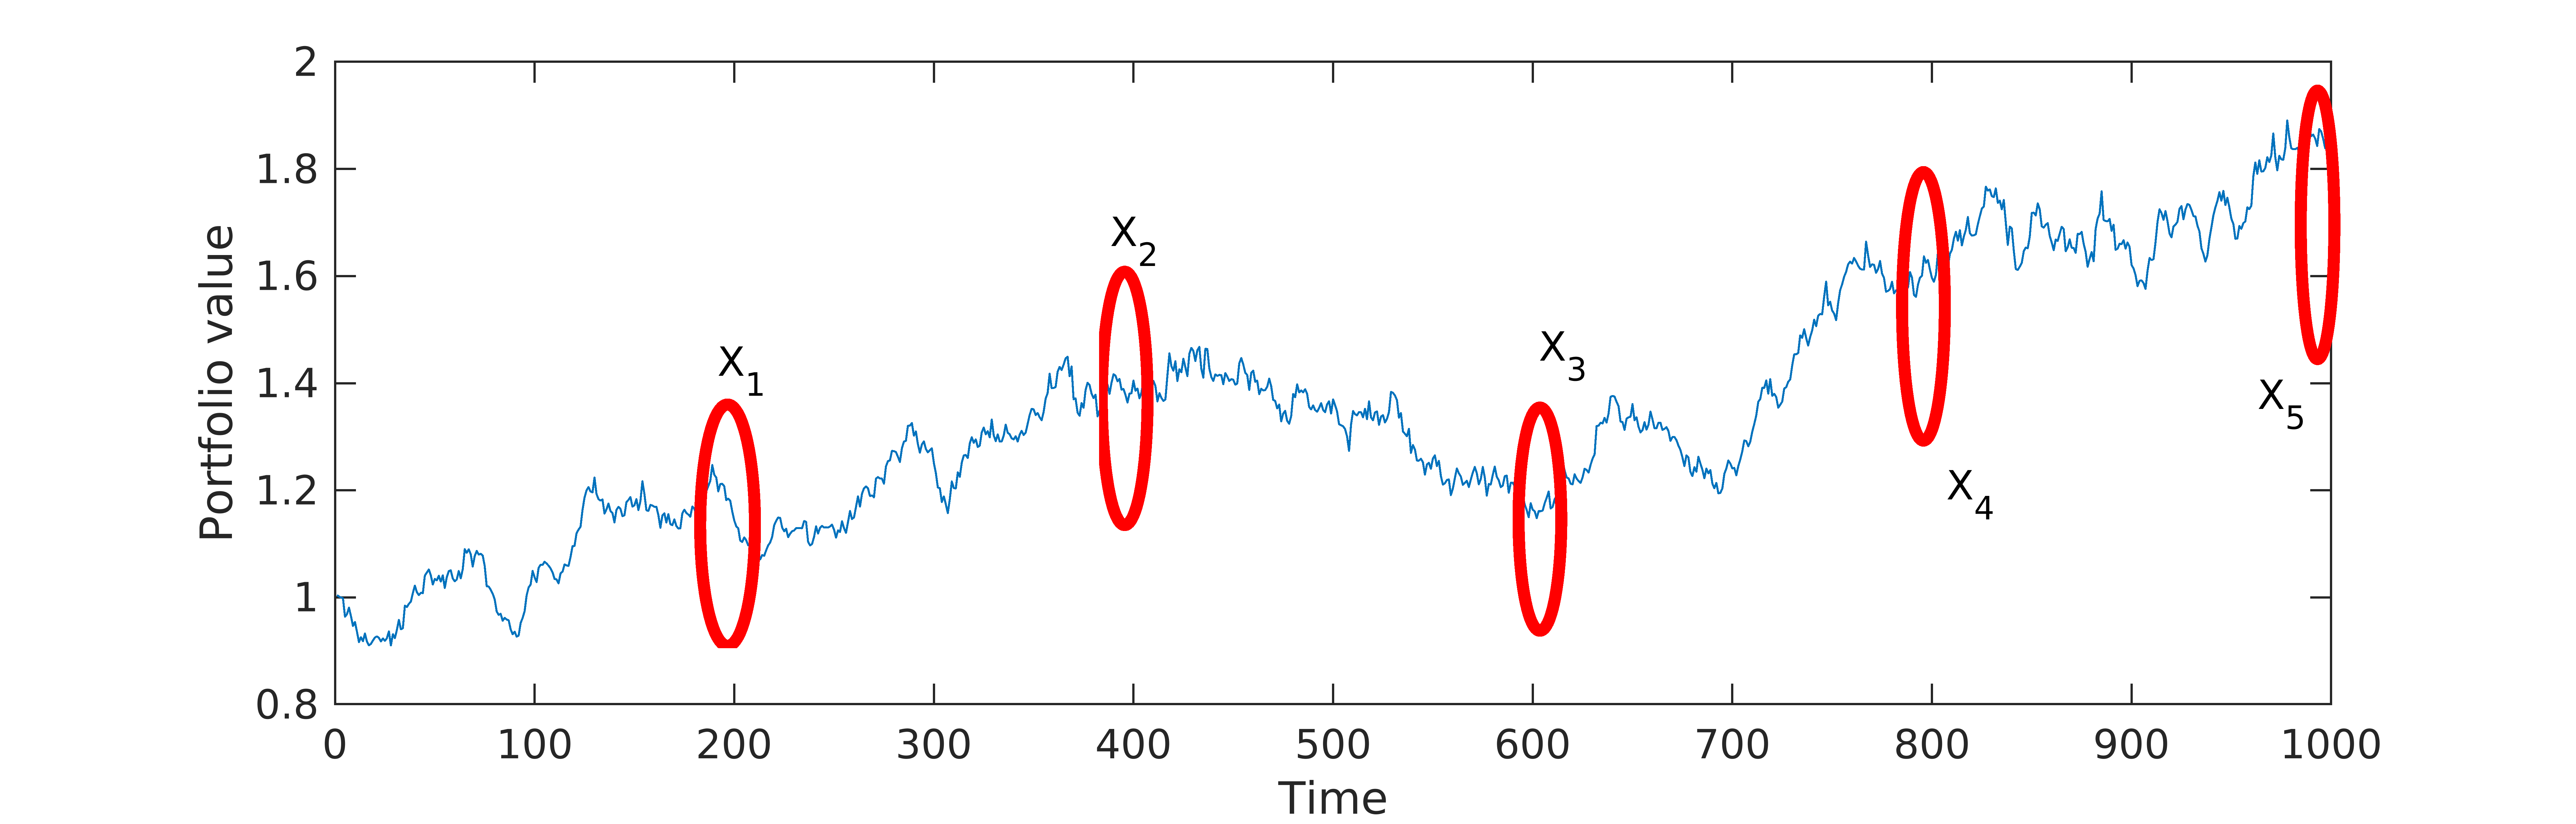
\includegraphics[width=1.1\linewidth]{Images/Reachability}
		\end{figure}

\end{frame}




	
	
\begin{frame}{}
	\frametitle{Piano della presentazione}
	\tableofcontents
\end{frame}	

	
\section{Approccio Time-Driven}
\begin{frame}{Modello matematico}
	\begin{block}{Dinamica di portafoglio}<1-2>
		\begin{equation*}
		x_{k+1} = x_k(1+\bm{u}_k^T\bm{w}_{k+1}), \quad k \in \mathbb{N}
		\end{equation*}
	\end{block}
	dove
	\begin{itemize}
		\item $x_k$ stato del sistema e valore del portafoglio al'istante $k\in \mathbb{N}$
		\item $\bm{u}_k$ variabile di controllo del sistema e vettore dei pesi di portafoglio
		\item $\bm{w}_{k+1}$ vettore dei rendimenti dei titoli
	\end{itemize}
	\begin{block}{Obiettivo}<2>
		\begin{equation*}
		\Optmax_{\pi \in \mathcal{U}_{N-1}} \mathbb{P}\Big(\big\{\omega \in \Omega : x_0 \in X_0,\ldots,x_N \in X_N \big\} \Big).
		\end{equation*}
	\end{block}
\end{frame}	


\begin{frame}{Modello Matematico}
	\begin{block}{Optimal Dynamic Asset Allocation (ODAA) Algorithm}
		\begin{align*}
		J_N(x) & = \mathbbm{1}_{X_N}(x) \nonumber \\
		J_k(x) & = \sup_{\bm{u}_k \in U_k}\int_{X_{k+1}}J_{k+1}(z)p_{f(x,\bm{u}_k,\bm{w}_{k+1})}(z)\mathrm{d}z \\
		& \forall k = N-1,\ldots,1,0. 
		\end{align*}
	\end{block}
    \begin{columns}
	    \begin{column}{.5\textwidth}
	    	In output l'algoritmo fornisce la \textbf{strategia ottima} 
	    	\[ \pi^{\star} =  \{\mu_0^{\star},\ldots,\mu_{N-1}^{\star} \},  \]
	    	ossia una sequenza di mappe \[  \mu_k^{\star} \colon x \mapsto \bm{u}_{k}^{\star}, \quad \forall k  \]
	    \end{column}
	    \begin{column}{.5\textwidth}<2>
	    	\begin{alertblock}{Elevato costo computazionale}
	    		un'ottimizzazione vincolata $\forall k = 1,\ldots,N-1, \quad \forall x \in X_k$
	    	\end{alertblock}
	    \end{column}
    \end{columns}
	
\end{frame}

\begin{frame}{Modello di mercato}
	I rendimenti delle asset class $\bm{w}_{k+1}$ vengono modellizzati con una \textbf{Mistura Gaussiana}:
	\begin{block}{}
		\begin{equation*}
		p_{\bm{w}_{k+1}} = \lambda\varphi_{(\bm{\mu_1},\bm{\Sigma}_1)} + (1-\lambda)\varphi_{(\bm{\mu_2},\bm{\Sigma}_2)}, \quad \lambda \in [0,1]
		\end{equation*}
	\end{block}
	\begin{figure}
		\centering
		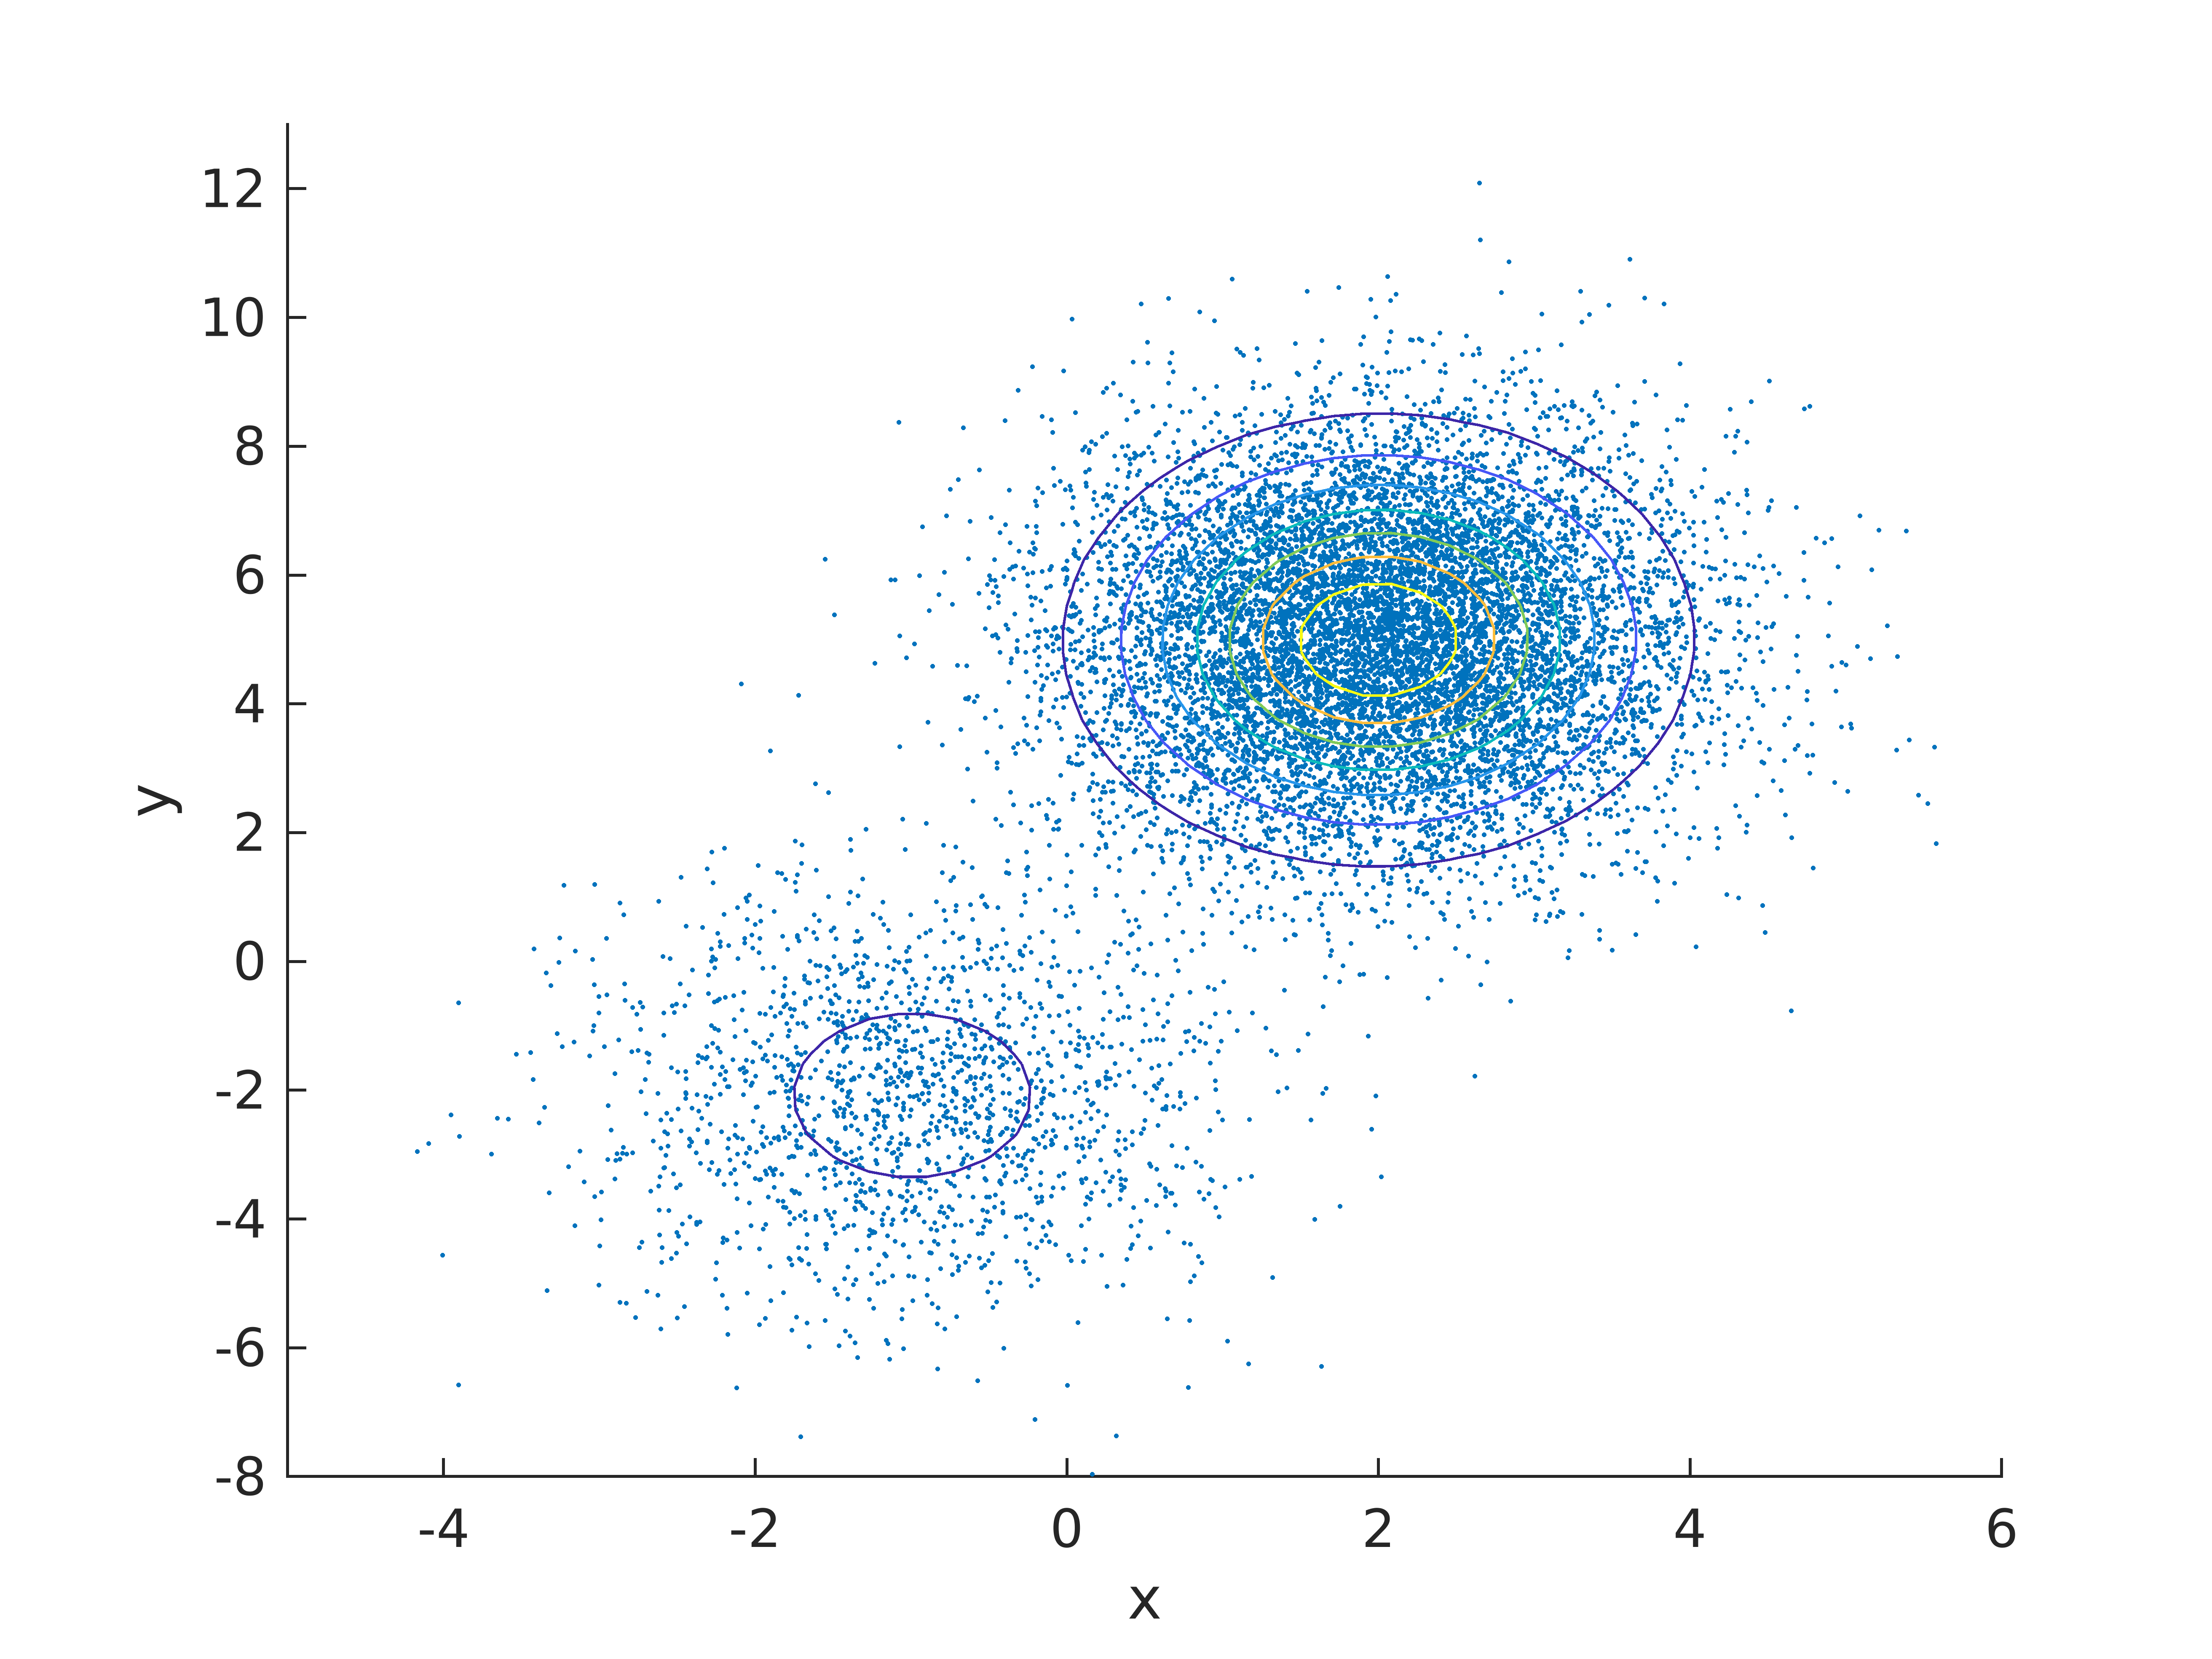
\includegraphics[width=0.65\linewidth]{Images/Scatter}
	\end{figure}
	
	
\end{frame}	

\begin{frame}{Mappe di Allocazione: }
	\begin{columns}
		\begin{column}{0.35\textwidth}
			\textbf{parametri investimento}:
				\begin{itemize}
					\item orizzonte 2 anni
					\item ribilanciamento settimanale
					\item  $x_0=1$
					\item target return 7\% annuo
					\item $V@R_{1-\alpha} = 7\%$
				\end{itemize}
			
			\textbf{probabilità raggiungimento target}:
			$p^{\star} = 78.59\%$
			
		\end{column}
		\begin{column}{0.65\textwidth}
			\begin{figure}
				\centering
				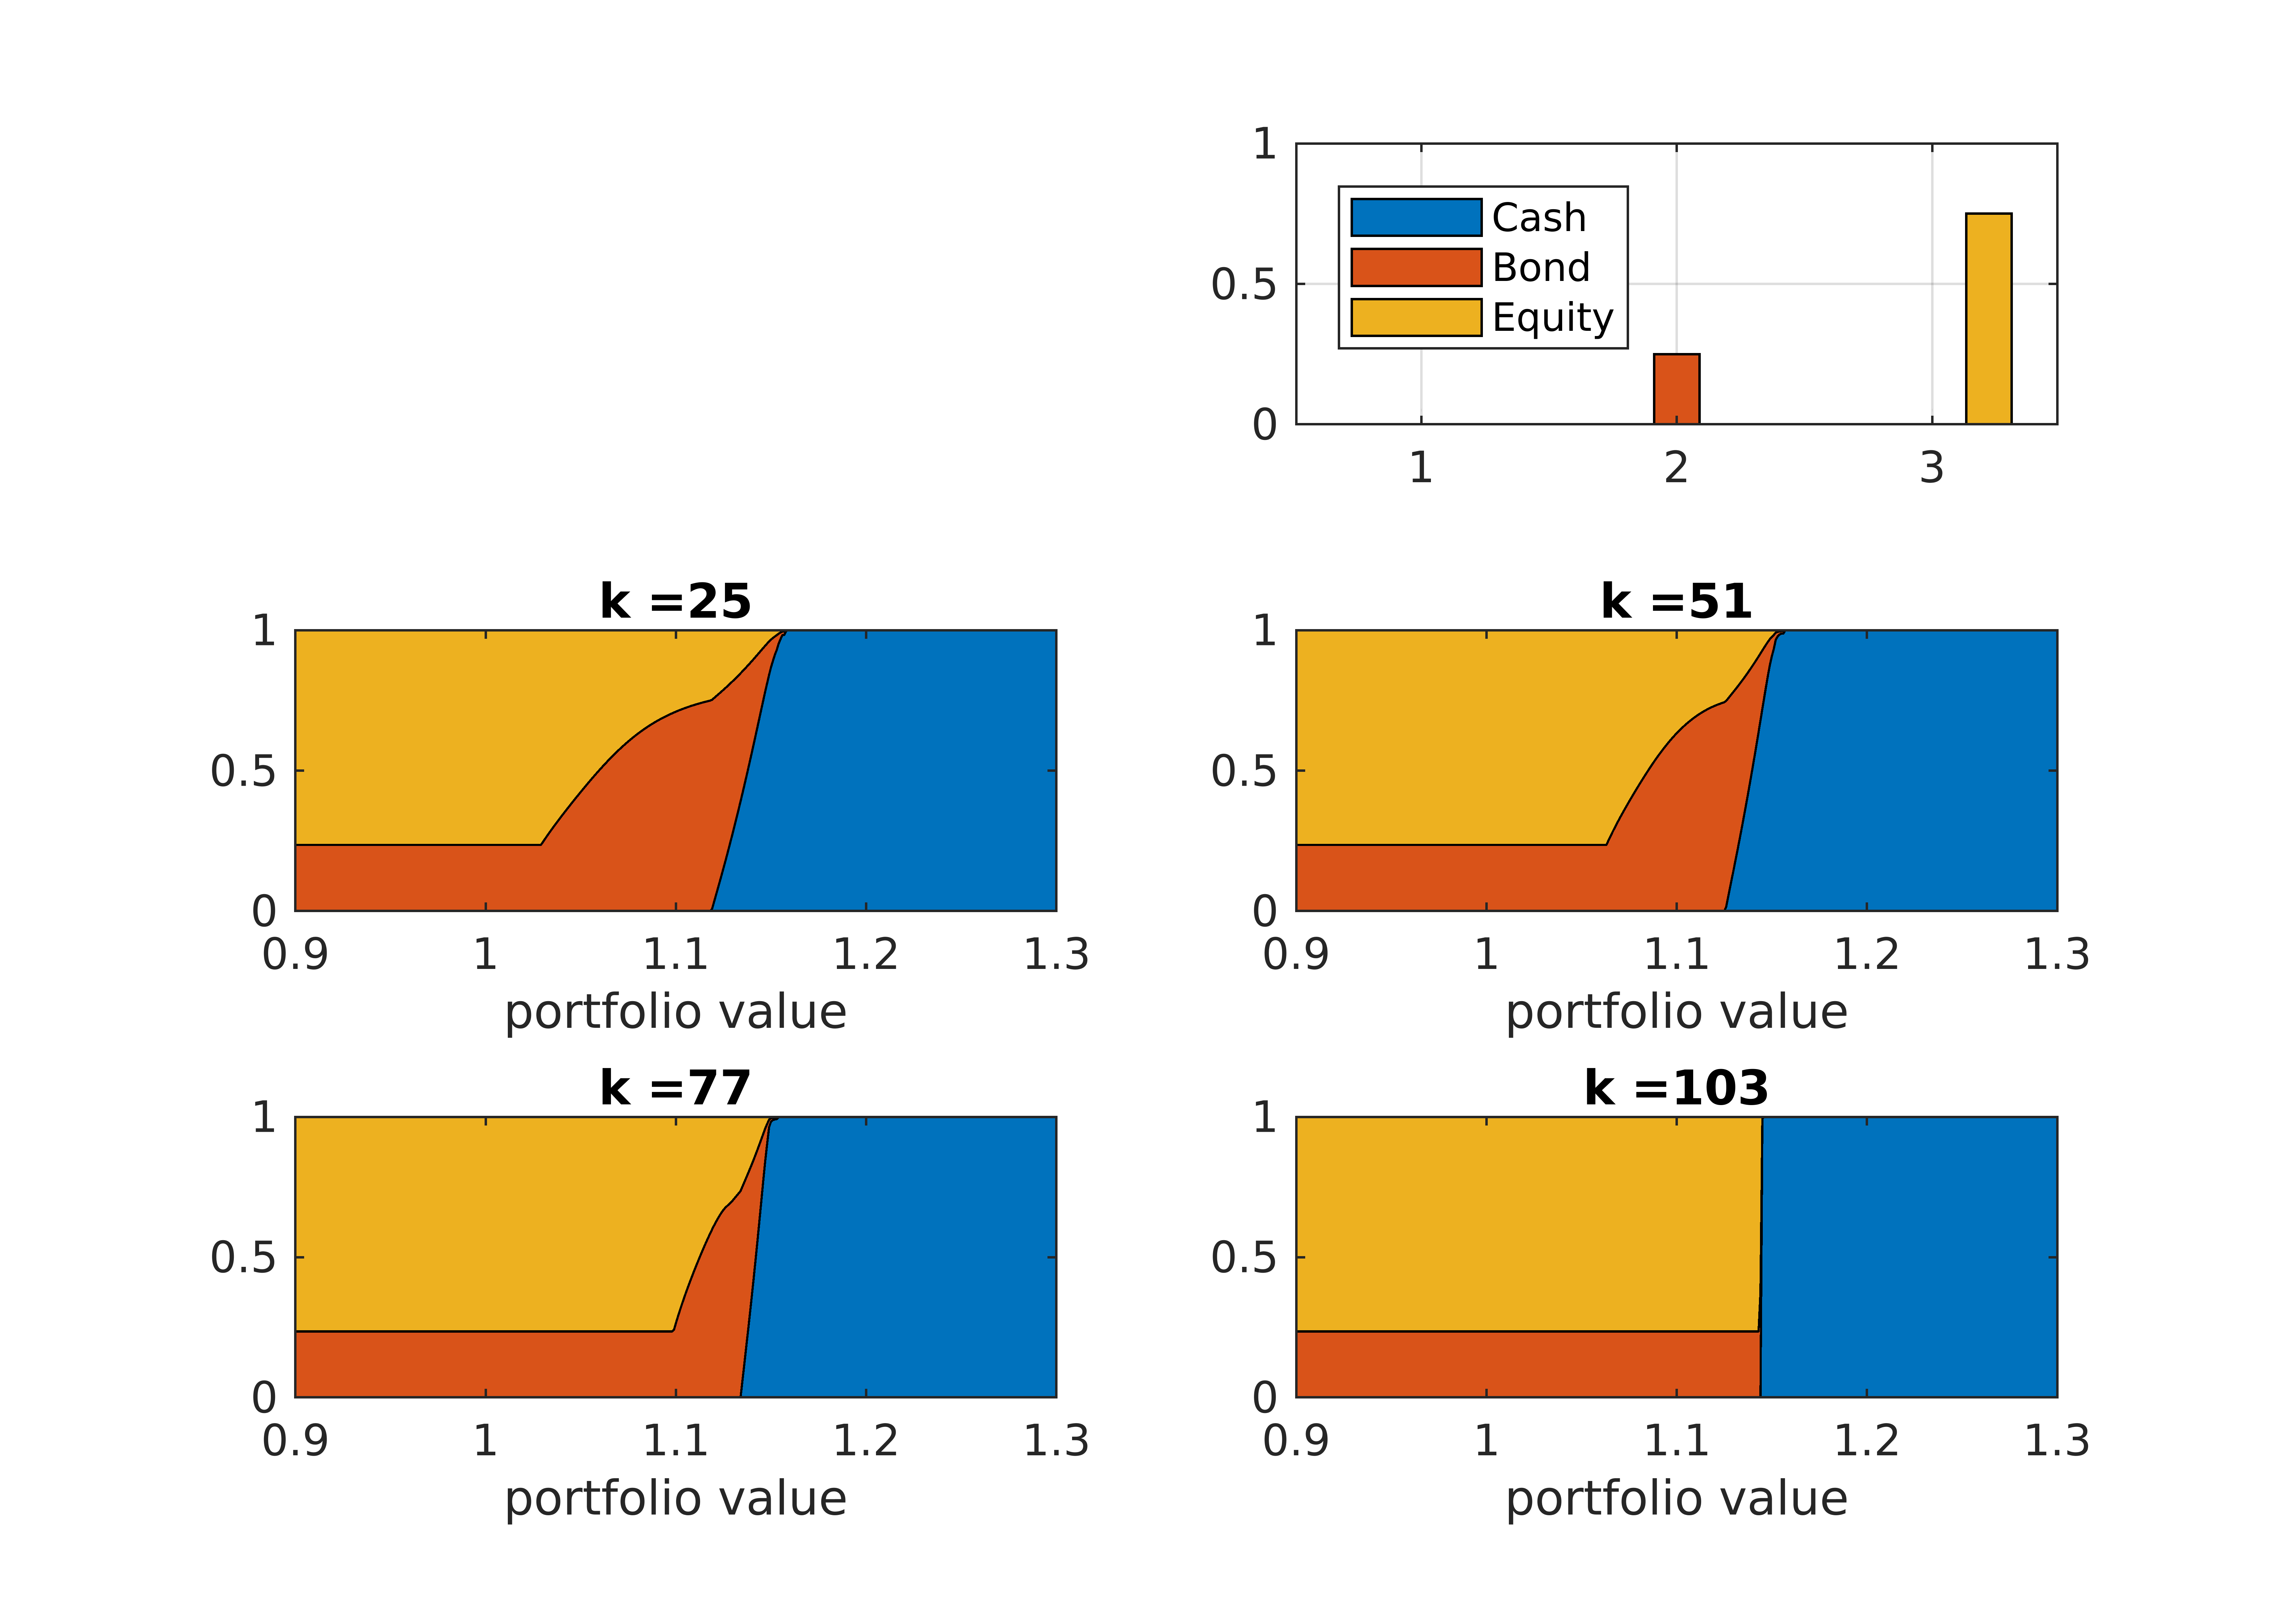
\includegraphics[height=5.5cm]{Images/mapsMixturewk}
			\end{figure}
		\end{column}
	\end{columns}
	
	
\end{frame}

\begin{frame}{Simulazione Monte Carlo}
	\begin{figure}
		\centering
		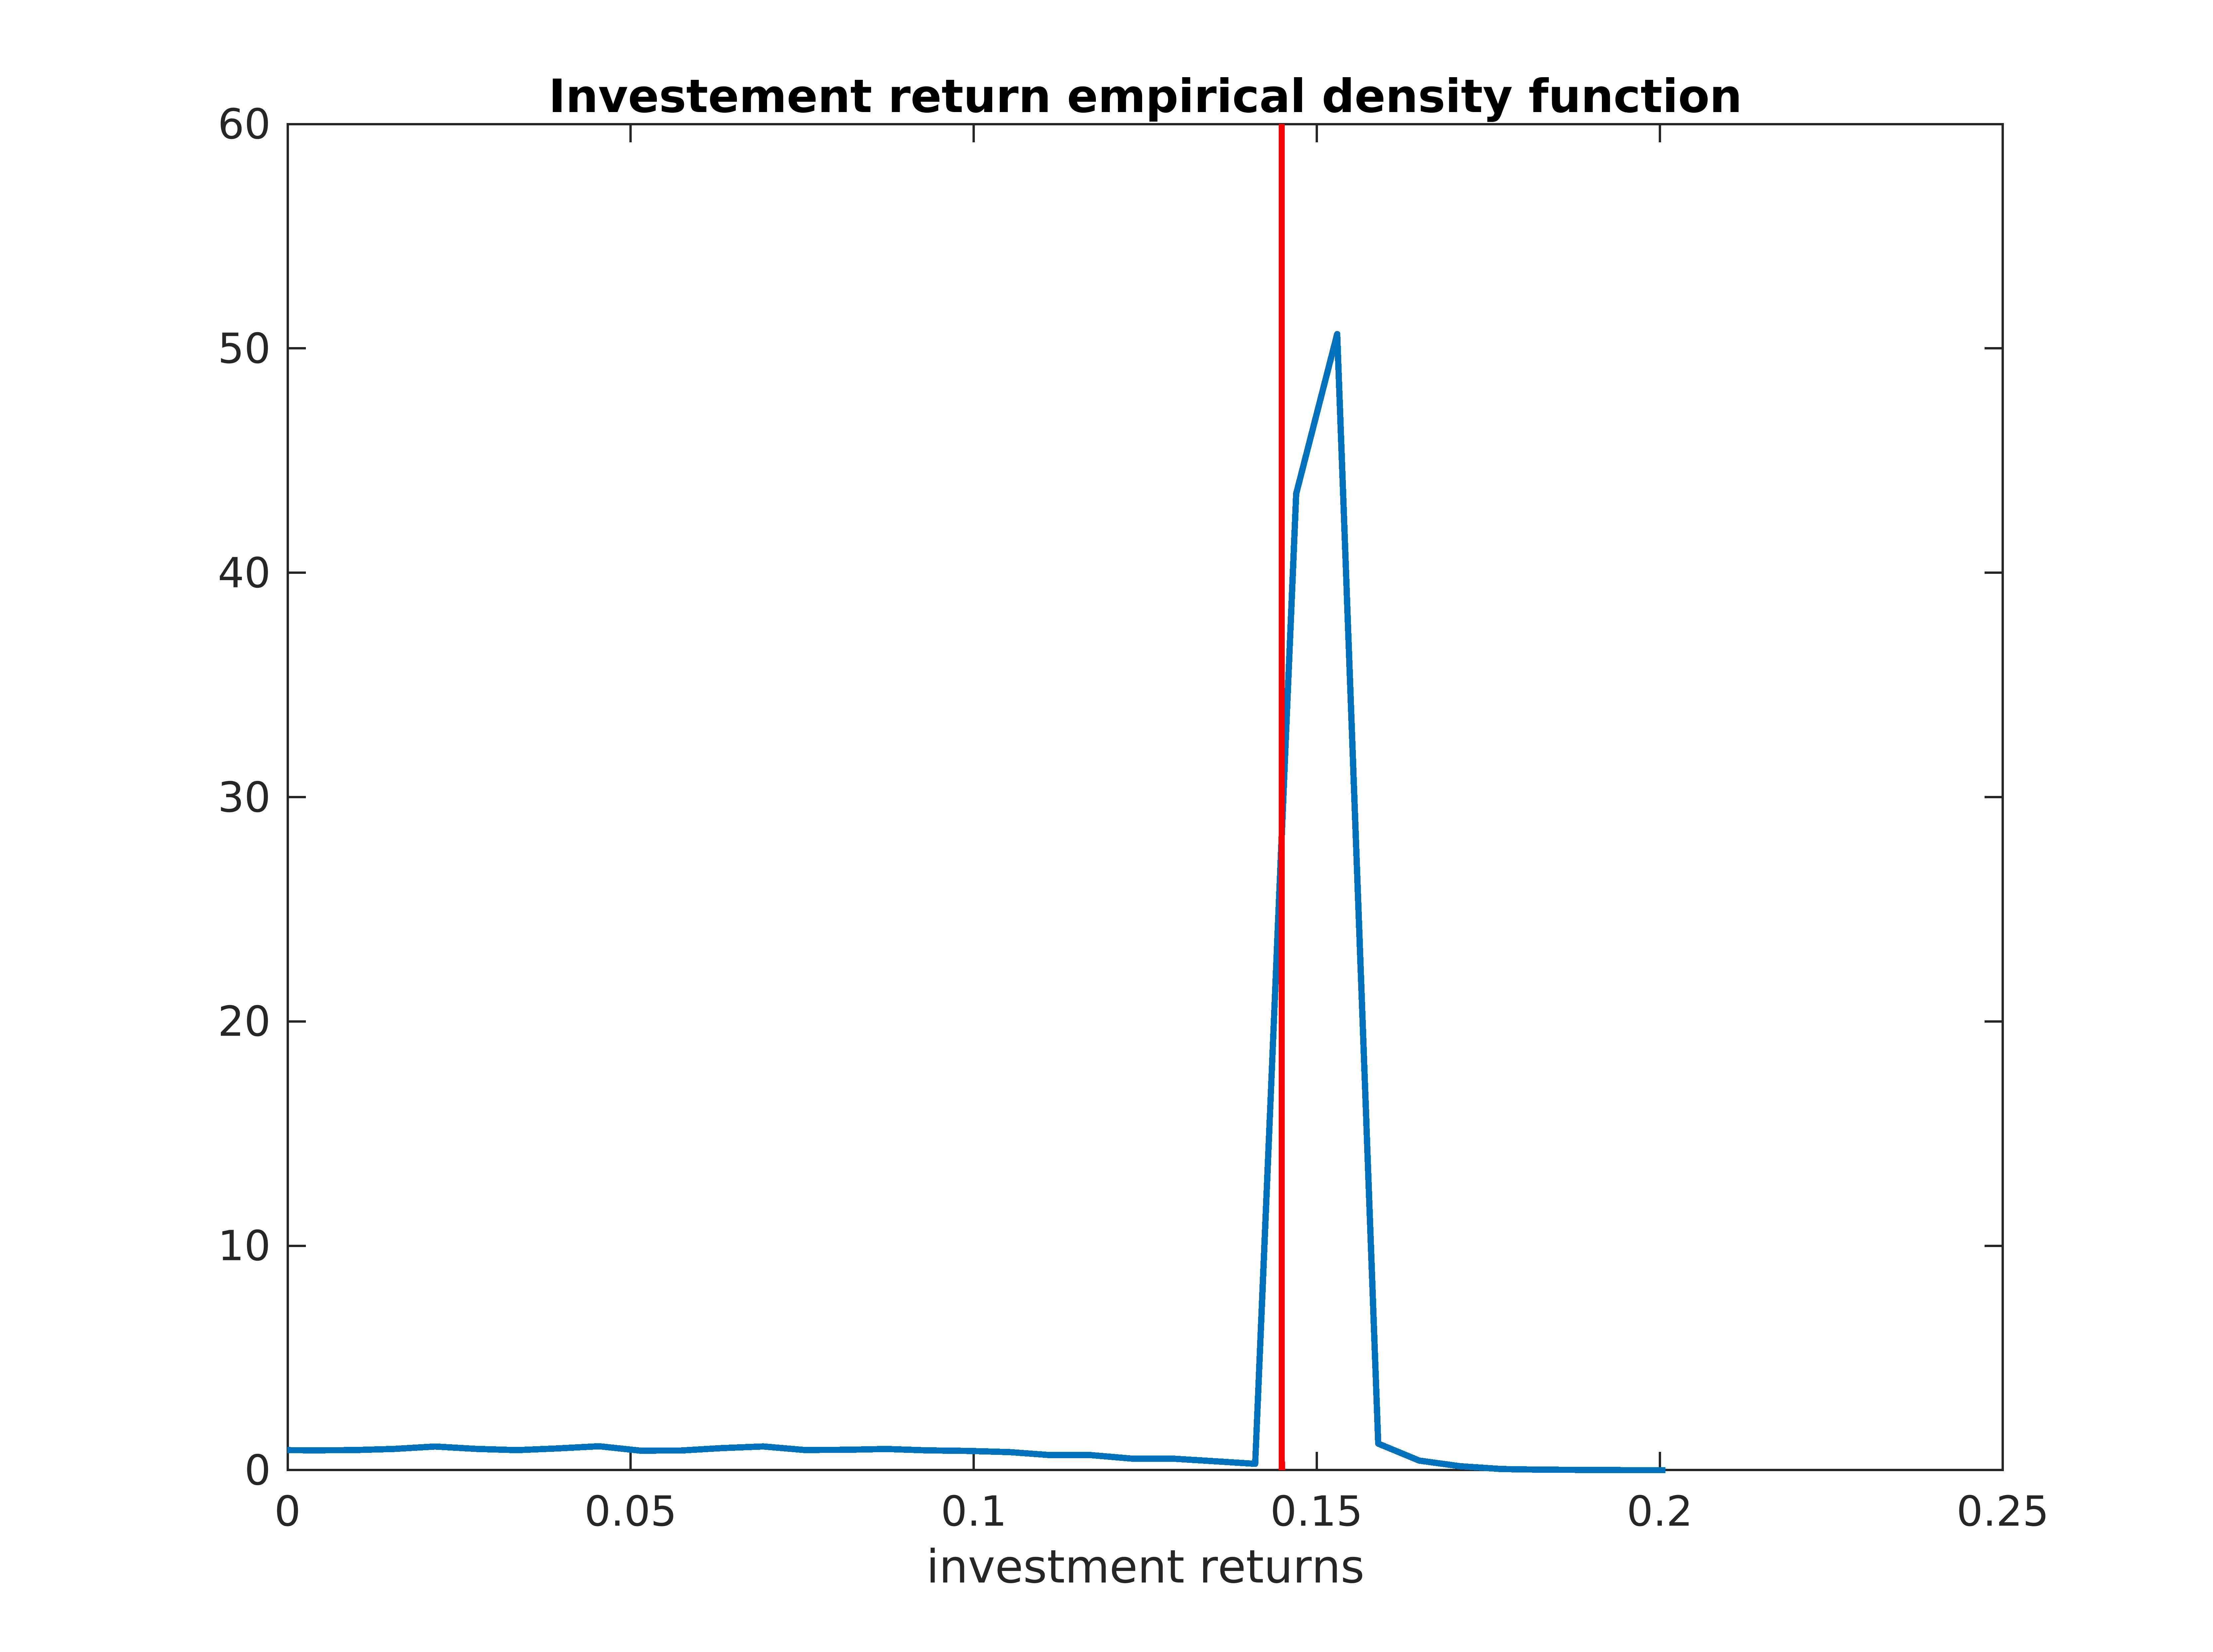
\includegraphics[width=0.8\linewidth]{Images/DensityODAAwk}
	\end{figure}
\end{frame}

	
\section{Approccio Event-Driven}


\begin{frame}{Definizione di "Evento"}
	\begin{definition}
		si dice che un \textbf{evento} è accaduto ogniqualvolta il rendimento cumulato dell'asset rischioso supera una prefissata soglia superiore o inferiore.
    \end{definition}
\begin{figure}
	\centering
	
\includegraphics[width=1.2\linewidth]{Images/ExitTime}
\end{figure}
\end{frame}	

\begin{frame}{Modello Event-Driven}
	\begin{columns}
		\begin{column}{.5\textwidth}
			\begin{block}{Dinamica del titolo rischioso}
				\begin{equation*}
				S_{k+1} = S_k(1+J\widetilde{N}_{k+1}), \quad k \in \mathbb{N}
				\end{equation*}
			\end{block}
			\begin{itemize}
				\item $J$ = ampiezza salto
				\item $\widetilde{N}_{k+1} \sim B(p)$
			\end{itemize}
		\end{column}
		\begin{column}{.5\textwidth}
			\begin{figure}
				\centering
				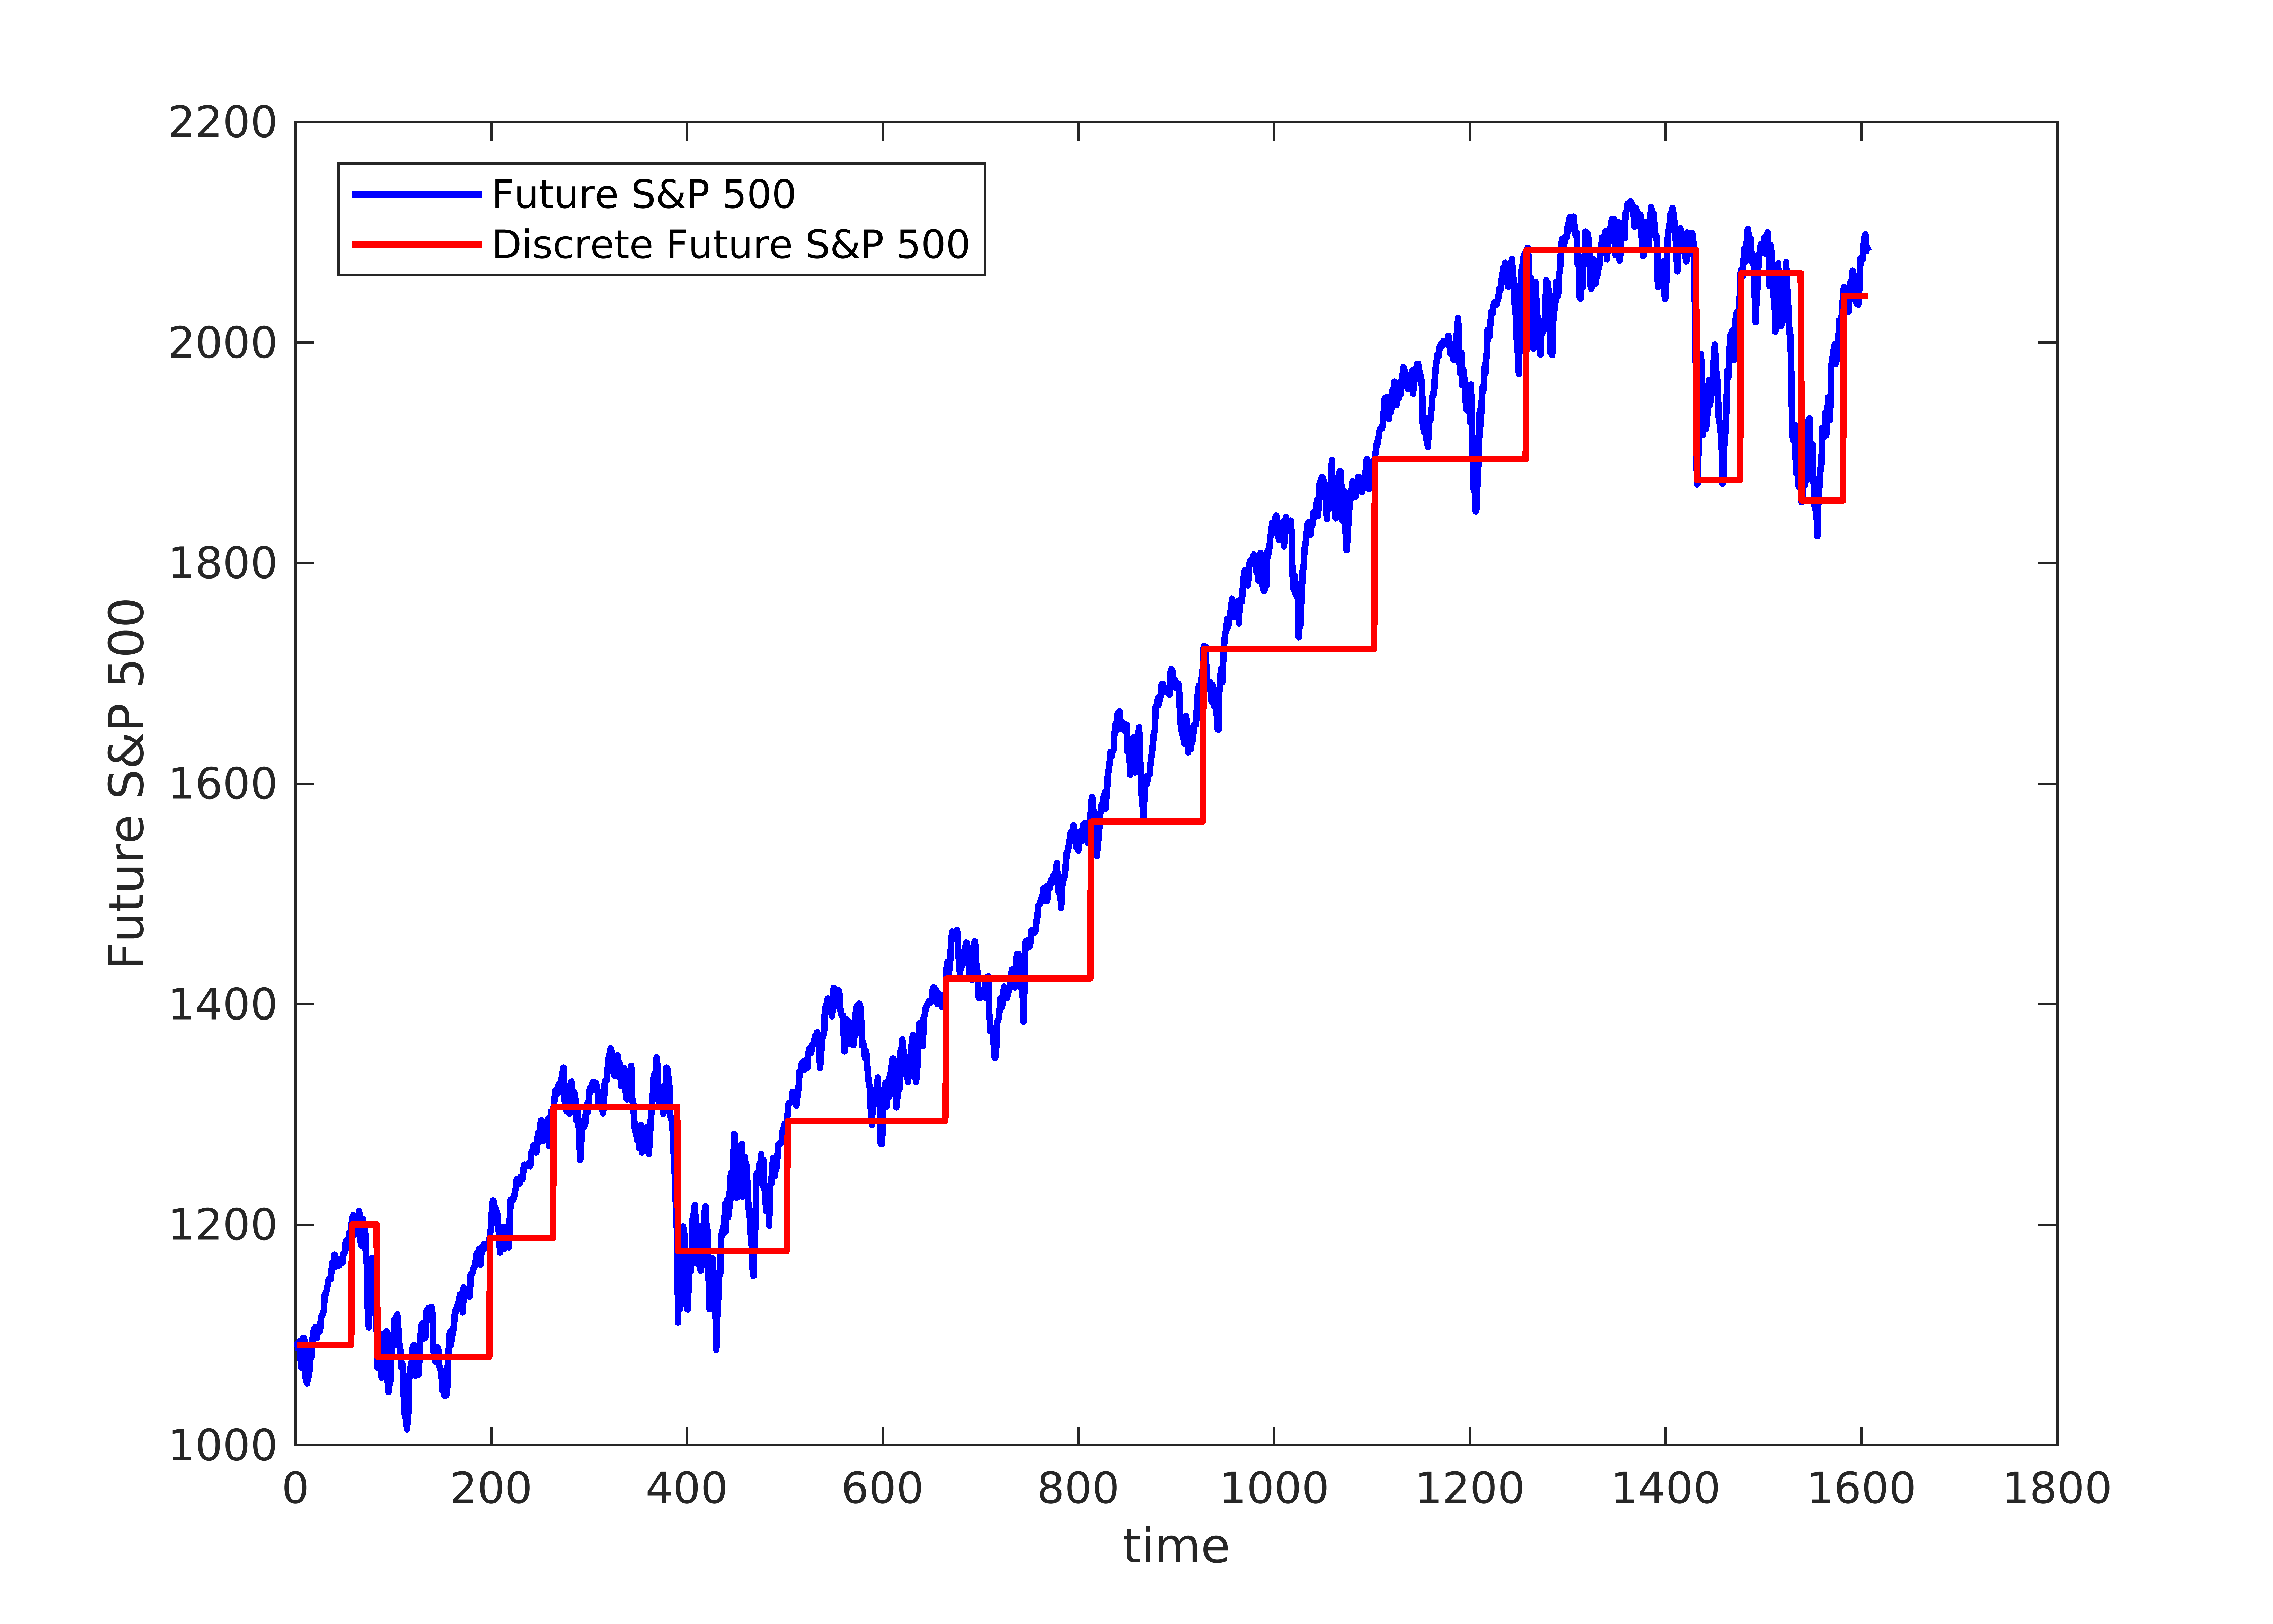
\includegraphics[width=1\linewidth]{Images/DiscreteDynamics}
			\end{figure}
		\end{column}
	\end{columns}
	\pause
	\begin{block}{Dinamica di Portafoglio}
		\begin{equation*}
		x_{k+1} = x_k(\exp\{r \tau_{k+1} \} + u_kJ\widetilde{N}_{k+1}), \quad k \in \mathbb{N}
		\end{equation*}
	\end{block}
	
\end{frame}






\begin{frame}{Mappe allocazione titolo rischioso}
	\begin{columns}
		\begin{column}{0.4\textwidth}
			\begin{block}{parametri investimento}
				\begin{itemize}
					\item 10 riallocazioni 
					\item $r=1\%$
					\item $X_{10} = [1.07^4,\infty]$
				\end{itemize}
			\end{block}
			\textbf{probabilità raggiungimento target}:
			$p^{\star}=73.5\%$
		\end{column}
		\begin{column}{0.6\textwidth}
			\begin{figure}
				\centering
				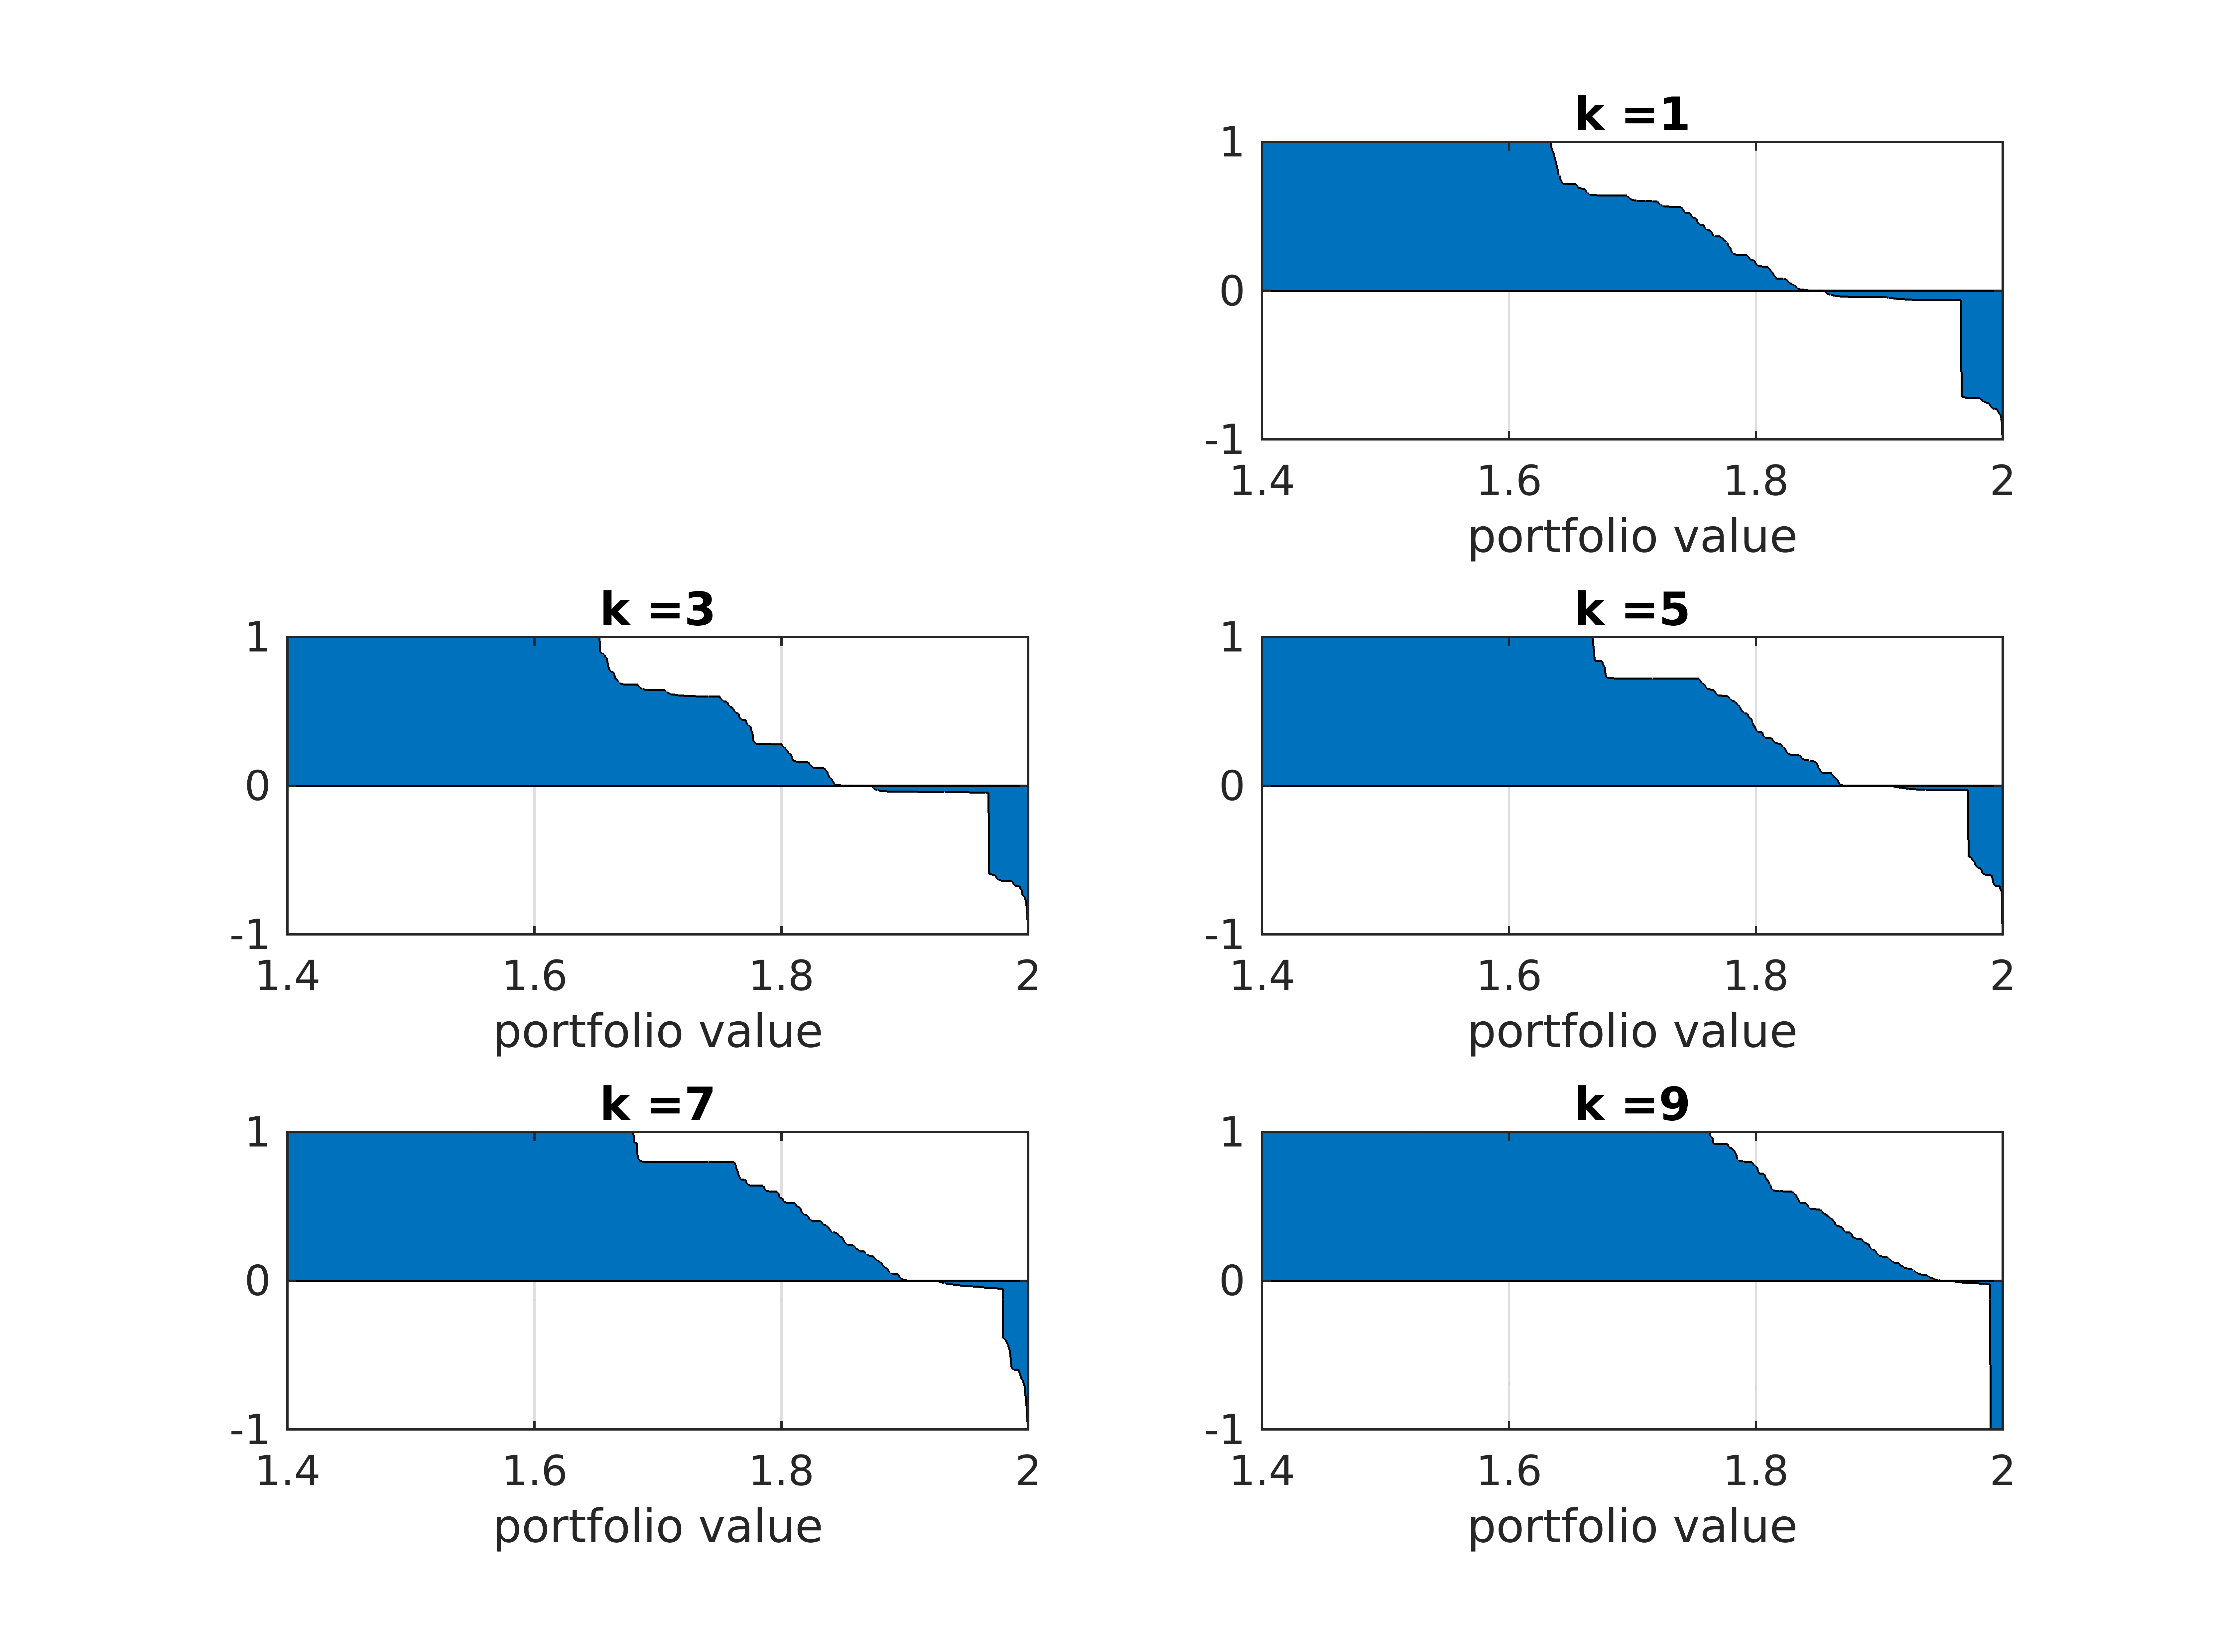
\includegraphics[width=1.1\linewidth]{Images/mapsbasic}
			\end{figure}
		\end{column}
	\end{columns}
\end{frame}

\begin{frame}{Estensione}
	
	
\end{frame}






\section{Conclusioni}
\textbf{Caratteristiche strategia ottima}:
	\begin{enumerate}
		\item multi-periodale
		\item indipendente da ipotesi distribuzionali sui rendimenti
	\end{enumerate}
%----------------------------------------------------------------------------------------
%	BODY
%----------------------------------------------------------------------------------------	
	
	
	
	
	
	
	
	
\end{document}